\begin{figure}[h!]
     \centering
    \captionsetup[sub]{font=small}
     \begin{subfigure}[b!]{0.43 \textwidth}
         \caption{}
         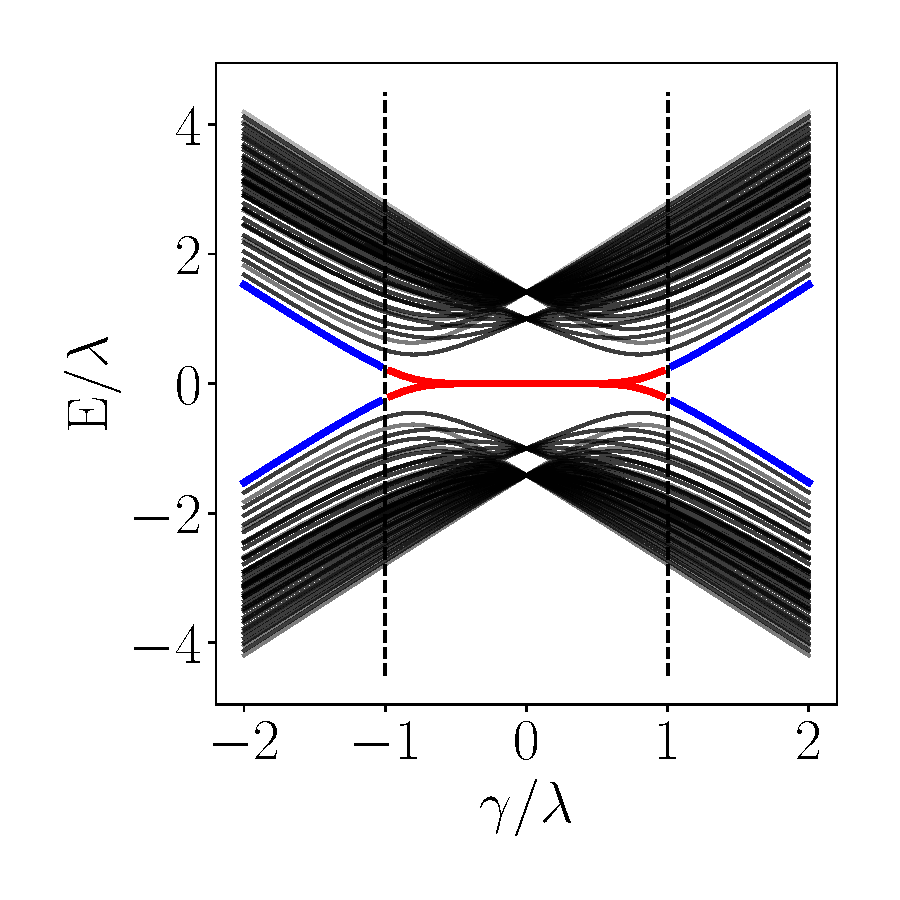
\includegraphics[width=\textwidth]{Imagenes/Resultados_Hoti_Cuadrado/bands_square_shh.pdf}
     \end{subfigure}
     \begin{subfigure}[b!]{0.56 \textwidth}
         \caption{}
         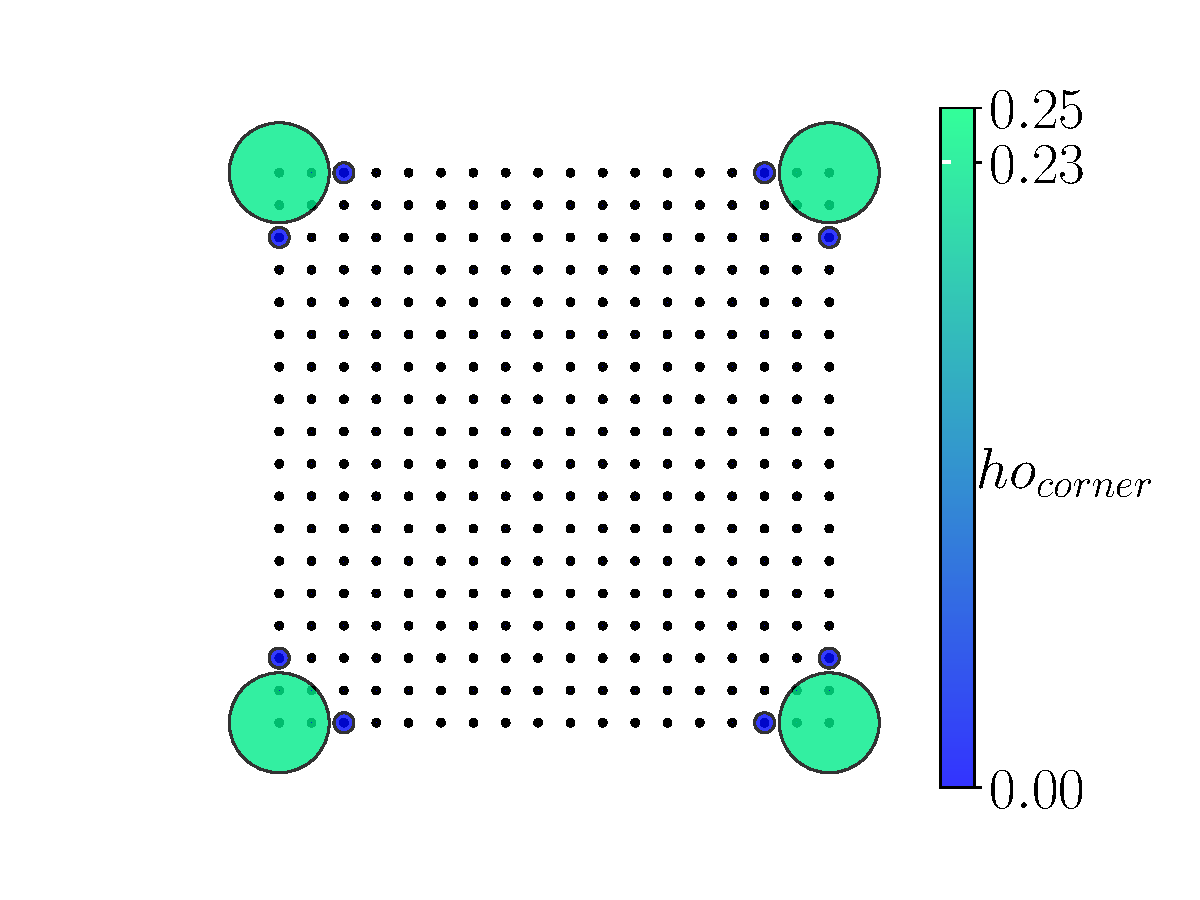
\includegraphics[width=\textwidth]{Imagenes/Resultados_Hoti_Cuadrado/proyection_square.pdf}
     \end{subfigure}\hspace*{1em} \vspace*{-0.5em}
        \caption{\textbf{(a)}Espectro de energía del sistema con geometría cuadrada y condiciones abiertas a la frontera, como función de $\gamma/\lambda$. Las energías de borde coloreadas en Azul-Rojo corresponde a los 4 estados localizados en las esquinas. \textbf{(b)} Densidad de probabilidad en un fase no trivial donde $\gamma = 0.5,\, \, \lambda = 1$, en un red cuadrada de $18\times18$ sitios.}
    \label{fig:Pram_Proy_cuadrado}
\end{figure}